W tym rozdziale przedstawiono przeprowadzone badania, sposób ich przeprowadzenia, przedstawiono sprzęt, na którym przeprowadzono badania.
\section{Opis komputera}
Wszystkie testy oraz badania zostały przeprowadzone na maszynie zaprezentowanej w tabeli \ref{tab:machine}. W tabeli wymieniono tylko znaczące elementy, tzn. procesor, pamięć RAM oraz jej szybkość, dysk twardy, jego prędkość obrotową oraz typ. Wszystkie te podzespoły mogą wpływać na czas trwania elementów działania aplikacji. Ze względu na jednowątkowość aplikacji, nie podaje się ilości wątków.
\begin{table}[H]
    \centering
    \begin{tabular}{|l|l|}
        \hline
        Procesor       & Intel Core-i5 8600 @ 3.10 GHz          \\ \hline
        Pamięć RAM     & 16GB DDR4 @ 3200 MHz \\ \hline
        Typ dysku twardego           & HDD              \\ \hline
        Dysk twardy         & Toshiba HDWD110              \\ \hline
        Prędkość obrotowa         & 7200 obr./min              \\ \hline
    \end{tabular}
    \caption{Spis części}
    \label{tab:machine}
\end{table}
Wszystkie pliki aplikacji zostały umieszczone na dysku HDD. Instancja baza danych znajduje się na dysku instalacyjnym, który jest rodzaju SSD.
\section{Parametry danych wejściowych}
\label{sec:entryparameters}
Dla każdego pliku umieszczonego w folderze \emph{\/data} w katalogu głównym aplikacji można określić następującą charakterystykę. Wykonane zostało 30 pomiarów punktu, w folderze istnieje 48 plików. Średnią ilością otrzymanych pomiarów, włącznie z punktami 'SS' jest XXX. Pomiary zostały wykonywane z częstotliwością 1000 Hz, czyli co 1 ms. W tabeli zaprezentowano indywidualną ilość pomiarów w każdym pliku.
\section{Przeprowadzone pomiary}
W tym podrozdziale zostaną zaprezentowane otrzymane wyniki, których format zaprezentowano w sekcji \ref{ssec:exitdata}. Dodatkowo do każdego wyniku została przygotowana krótka analiza wraz z zaprezentowaniem dopełniających parametrów wyników, umożliwiających lepszą interpretację rezultatów. Pierwszym elementem jest ukazanie wpływu parametrów wewnętrznych algorytmów na wyniki końcowe. Druga sekcja porównuje czasy trwania algorytmów, wraz z analizą przyczyn różnic czasowych. Następna sekcja opisuje wyniki obciążenia pamięciowego przez zaimplementowane algorytmy wykrywania fiksacji, jak również opisuje najbardziej obciążające metody. W przedostatnim podrozdziale zanalizowano metody wprowadzania danych wejściowych do aplikacji. Ostatnia analiza dotyczy dokładności algorytmu uczenia maszynowego oraz porównania wynikowych punktów wszystkich trzech algorytmów przedstawionych w sekcji \ref{ssec:algorithms}.
\subsection{Analiza wpływu parametrów algorytmów}
\label{ssec:queryparameters}
W poniższej sekcji zostanie zaprezentowany wpływ parametrów wewnętrznych algorytmów opisanych w sekcji \ref{ssec:algorithms}. Zbadany zostanie ten wpływ pod kątem różnic w obciązeniu pamięciowym przez algorytmy, porównania ilości elementów wyjściowych oraz czasu trwania algorytmów. Ten podrozdział został podzielony na 3 części, każda prezentująca algorytmy opisane w sekcji \ref{ssec:algorithms}. W celu prezentacji wyników wykorzystano pierwszych dziesięć plików opisanych w sekcji \ref{sec:entryparameters}.
\subsubsection{Algorytm I-VT}
\label{sssec:ivtresults}
Algorytm I-VT możemy zbadać pod kątem wpływu parametru granicznej prędkości międzypunktowej. Celem tej sekcji jest prezentacja otrzymanych wyników, wraz z krótką analizą.\par
\textbf{Liczba wykrytych fiksacji}\par
W tabeli \ref{tab:ivtfixationcomparison} zaprezentowano wynik pomiaru ilości wykrytych fiksacji przeprowadzonej na dziesięciu plikach dla algorytmu I-VT. W pierwszej kolumnie umieszczono nazwę pliku, a w następnych pomiar ilości, wraz z parametrem prędkości międzypunktowej.\\
Jak można zauważyć dla tego algorytmu im mniejsza prędkość graniczna, tym więcej punktów jest wykrywanych. Im mniejszy parametr tym mniej dokładnie filtrowane są punkty, co może spowodować sytuację zaprezentowaną na rysunku \ref{fig:ivterrorresults}, gdzie możemy zaobserwować duży spadek w dokładności zmierzonych fiksacji.
Jest to wynikiem porównania zaprezentowanego w pseudokodzie \ref{lst:ivtpseudocode}, więc można stwierdzić, iż wyniki algorytmu są zgodne z oczekiwaniami.\\
Po zaobserwowaniu wyników graficznych w plikach wynikowych stwierdzono, iż parametr prędkości powinien znajdować się w okolicach wartości $v \in (0,005)$, gdyż dla tego wyniku zaobserwowano najdokładniejsze wyniki. Ostatnią wartością badaną było $v = 0,1$, jednak dla tego parametru wynikiem było od 0 do 1 fiksacji, dlatego został on pominięty w tabeli wynikowej.\par
\begin{figure}[H]
    \centering
    \captionsetup{justification=centering,margin=2cm}
    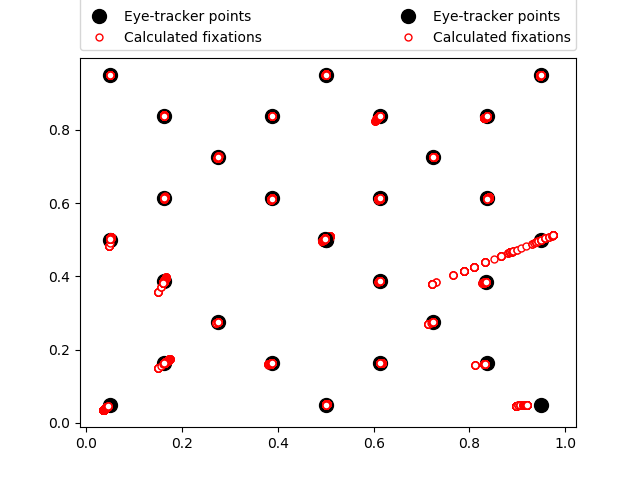
\includegraphics[width=\linewidth]{resources/ivt-errorresults.png}
    \caption{Błędne przedstawienie punktów dla algorytmu I-VT}
    \label{fig:ivterrorresults}
\end{figure}
{\small
\begin{longtable}{l|l|l|l|l|l|l|l|l|} 
    \cline{2-9}
     & \multicolumn{8}{c|}{\textbf{Ilość fiksacji/sakad}} \\ \hline
    \endfirsthead
    %
    \multicolumn{9}{c}%
    {{\bfseries Kontynuacja tabeli \thetable\ }} \\
    \cline{2-9}
     & \multicolumn{8}{c|}{\textbf{Ilość fiksacji/sakad}} \\ \hline
    \endhead
    %
    \multicolumn{1}{|c|}{\textbf{Plik}} & \multicolumn{2}{c|}{\textbf{v = 0,0001}} & \multicolumn{2}{c|}{\textbf{v = 0,005}} & \multicolumn{2}{c|}{\textbf{v = 0,001}} & \multicolumn{2}{l|}{\textbf{v = 0,01}} \\ \hline
    \multicolumn{1}{|l|}{1\_01\_1311201811.cal} & 6434 & \cellcolor[HTML]{EFEFEF}91444 & 780 & \cellcolor[HTML]{EFEFEF}3744 & 18015 & \cellcolor[HTML]{EFEFEF}52054 & 513 & \cellcolor[HTML]{EFEFEF}1545 \\ \hline
    \multicolumn{1}{|l|}{1\_02\_1310301856.cal} & 5896 & \cellcolor[HTML]{EFEFEF}92107 & 110 & \cellcolor[HTML]{EFEFEF}2415 & 1011 & \cellcolor[HTML]{EFEFEF}8817 & 37 & \cellcolor[HTML]{EFEFEF}405 \\ \hline
    \multicolumn{1}{|l|}{1\_03\_1310301904.cal} & 5645 & \cellcolor[HTML]{EFEFEF}92313 & 99 & \cellcolor[HTML]{EFEFEF}2027 & 1592 & \cellcolor[HTML]{EFEFEF}7547 & 54 & \cellcolor[HTML]{EFEFEF}446 \\ \hline
    \multicolumn{1}{|l|}{1\_04\_1310301810.cal} & 6792 & \cellcolor[HTML]{EFEFEF}90736 & 101 & \cellcolor[HTML]{EFEFEF}1688 & 1526 & \cellcolor[HTML]{EFEFEF}9217 & 30 & \cellcolor[HTML]{EFEFEF}263 \\ \hline
    \multicolumn{1}{|l|}{1\_05\_1310301817.cal} & 6475 & \cellcolor[HTML]{EFEFEF}91476 & 204 & \cellcolor[HTML]{EFEFEF}2877 & 11015 & \cellcolor[HTML]{EFEFEF}25880 & 85 & \cellcolor[HTML]{EFEFEF}939 \\ \hline
    \multicolumn{1}{|l|}{1\_06\_1310301837.cal} & 6815 & \cellcolor[HTML]{EFEFEF}90960 & 98 & \cellcolor[HTML]{EFEFEF}1889 & 3308 & \cellcolor[HTML]{EFEFEF}8590 & 42 & \cellcolor[HTML]{EFEFEF}288 \\ \hline
    \multicolumn{1}{|l|}{1\_12\_1310301901.cal} & 6726 & \cellcolor[HTML]{EFEFEF}91100 & 118 & \cellcolor[HTML]{EFEFEF}1865 & 6954 & \cellcolor[HTML]{EFEFEF}14511 & 42 & \cellcolor[HTML]{EFEFEF}399 \\ \hline
    \multicolumn{1}{|l|}{1\_14\_1310301912.cal} & 11964 & \cellcolor[HTML]{EFEFEF}82189 & 83 & \cellcolor[HTML]{EFEFEF}2213 & 278 & \cellcolor[HTML]{EFEFEF}6612 & 46 & \cellcolor[HTML]{EFEFEF}641 \\ \hline
    \multicolumn{1}{|l|}{1\_15\_1310301840.cal} & 7737 & \cellcolor[HTML]{EFEFEF}89751 & 87 & \cellcolor[HTML]{EFEFEF}1208 & 12041 & \cellcolor[HTML]{EFEFEF}22008 & 42 & \cellcolor[HTML]{EFEFEF}263 \\ \hline
    \multicolumn{1}{|l|}{1\_16\_1310301844.cal} & 6509 & \cellcolor[HTML]{EFEFEF}91431 & 126 & \cellcolor[HTML]{EFEFEF}1745 & 17453 & \cellcolor[HTML]{EFEFEF}42023 & 48 & \cellcolor[HTML]{EFEFEF}529 \\ \hline
    \caption{Wpływ parametru prędkości granicznej dla algorytmu I-VT, ilość fiksacji}
    \label{tab:ivtfixationcomparison}\\
\end{longtable}
}
\textbf{Analiza czasu trwania algorytmu}\par
W tabeli \ref{tab:ivttimecomparison} zaprezentowano wyniki pomiaru czasu trwania algorytmu I-VT. Czas trwania zaprezentowano w sekundach. Obserwując otrzymane wyniki możemy określić, iż czas trwania algorytmu wzrasta odwrotnie proporcjonalnie do ilości wykrytych fiksacji. Zastanawiającym wynikiem jest pomiar czasu dla parametru $v = 0,01$, ze względu na swoje podobieństwo do rezultatów z pierwszej kolumny. Jest to spowodowane małą ilością elementów koniecznych do wykonania drugiego porównania, ze względu na duży parametr prędkości.\par
{\small
\begin{longtable}{l|l|l|l|l|}
    \cline{2-5}
     & \multicolumn{4}{c|}{\textbf{Pomiar długości trwania algorytmu (w s)}} \\ \hline
    \endfirsthead
    %
    \multicolumn{5}{c}%
    {{\bfseries Kontynuacja tabeli \thetable\ }} \\
    \cline{2-5}
     & \multicolumn{4}{c|}{\textbf{Pomiar długości trwania algorytmu (w s)}} \\ \hline
    \endhead
    %
    \multicolumn{1}{|c|}{\textbf{Plik}} & \multicolumn{1}{c|}{\textbf{v = 0,0001}} & \multicolumn{1}{c|}{\textbf{v = 0,005}} & \multicolumn{1}{c|}{\textbf{v = 0,001}} & \textbf{v = 0,01} \\ \hline
    \multicolumn{1}{|l|}{1\_01\_1311201811.cal} & 1.265625 & 4.21875 & 24.234375 & 3.515625 \\ \hline
    \multicolumn{1}{|l|}{1\_02\_1310301856.cal} & 1.203125 & 1.671875 & 4.375 & 1.5625 \\ \hline
    \multicolumn{1}{|l|}{1\_03\_1310301904.cal} & 1.15625 & 1.5625 & 6.203125 & 1.46875 \\ \hline
    \multicolumn{1}{|l|}{1\_04\_1310301810.cal} & 1.578125 & 1.546875 & 6.0625 & 1.5 \\ \hline
    \multicolumn{1}{|l|}{1\_05\_1310301817.cal} & 1.203125 & 1.921875 & 31.765625 & 1.625 \\ \hline
    \multicolumn{1}{|l|}{1\_06\_1310301837.cal} & 1.25 & 1.53125 & 12.3125 & 1.4375 \\ \hline
    \multicolumn{1}{|l|}{1\_12\_1310301901.cal} & 1.359375 & 1.546875 & 24.875 & 1.4375 \\ \hline
    \multicolumn{1}{|l|}{1\_14\_1310301912.cal} & 4.203125 & 1.484375 & 1.90625 & 1.5 \\ \hline
    \multicolumn{1}{|l|}{1\_15\_1310301840.cal} & 1.421875 & 1.421875 & 33.875 & 1.421875 \\ \hline
    \multicolumn{1}{|l|}{1\_16\_1310301844.cal} & 1.140625 & 1.46875 & 34.5625 & 1.453125 \\ \hline
    \caption{Wpływ parametru prędkości granicznej dla algorytmu I-VT, pomiar czasu}
    \label{tab:ivttimecomparison}\\
\end{longtable}
}
\textbf{Analiza wykorzystania pamięci operacyjnej}\par
Tabela \ref{tab:ivtmemorycomparison} przedstawia wyniki analizy wykorzystania pamięci przez algorytm I-VT. Jednostką pomiaru jest MiB. Zgodnie z zaobserwowanymi pomiarami, można stwierdzić, iż dla obecnych maszyn pomiar algorytmem I-VT nie stanowi zbytniego obciążenia, gdyż pomiary oscylują pomiędzy setkami a dziesiątkami kilobajtów na cały pomiar. Nie zauważono znaczącego wpływu parametru algorytmu na wykorzystanie pamięciowe, bo jak można zaobserwować, liczba otrzymanych elementów nie ma wpływu na zużycie pamięci operacyjnej.\par
{\small
\begin{longtable}{l|l|l|l|l|}
    \cline{2-5}
     & \multicolumn{4}{c|}{\textbf{\begin{tabular}[c]{@{}c@{}}Wykorzystanie pamięci operacyjnej\\  (w MiB)\end{tabular}}} \\ \hline
    \endfirsthead
    %
    \multicolumn{5}{c}%
    {{\bfseries Kontynuacja tabeli \thetable\ }} \\
    \cline{2-5}
     & \multicolumn{4}{c|}{\textbf{\begin{tabular}[c]{@{}c@{}}Wykorzystanie pamięci operacyjnej\\  (w MiB)\end{tabular}}} \\ \hline
    \endhead
    %
    \multicolumn{1}{|c|}{\textbf{Plik}} & \multicolumn{1}{c|}{\textbf{v = 0,0001}} & \multicolumn{1}{c|}{\textbf{v = 0,005}} & \multicolumn{1}{c|}{\textbf{v = 0,001}} & \textbf{v = 0,01} \\ \hline
    \multicolumn{1}{|l|}{1\_01\_1311201811.cal} & 0.12500 & 0.17188 & 0.15234 & 0.21094 \\ \hline
    \multicolumn{1}{|l|}{1\_02\_1310301856.cal} & 0.10156 & 0.24609 & 0.16797 & 0.18359 \\ \hline
    \multicolumn{1}{|l|}{1\_03\_1310301904.cal} & 0.16016 & 0.15234 & 0.13281 & 0.12891 \\ \hline
    \multicolumn{1}{|l|}{1\_04\_1310301810.cal} & 0.19531 & 0.17188 & 0.12500 & 0.15625 \\ \hline
    \multicolumn{1}{|l|}{1\_05\_1310301817.cal} & 0.12109 & 0.15625 & 0.16406 & 0.24219 \\ \hline
    \multicolumn{1}{|l|}{1\_06\_1310301837.cal} & 0.06641 & 0.11328 & 0.12500 & 0.25000 \\ \hline
    \multicolumn{1}{|l|}{1\_12\_1310301901.cal} & 0.12500 & 0.22656 & 0.24219 & 0.17188 \\ \hline
    \multicolumn{1}{|l|}{1\_14\_1310301912.cal} & 0.20313 & 0.18750 & 0.21094 & 0.16016 \\ \hline
    \multicolumn{1}{|l|}{1\_15\_1310301840.cal} & 0.12109 & 0.12891 & 0.12891 & 0.21094 \\ \hline
    \multicolumn{1}{|l|}{1\_16\_1310301844.cal} & 0.10156 & 0.19922 & 0.17969 & 0.16797 \\ \hline
    \caption{Wpływ parametru prędkości granicznej dla algorytmu I-VT, wykorzystanie pamięci operacyjnej}
    \label{tab:ivtmemorycomparison}\\
\end{longtable}
}
\subsubsection{Algorytm I-DT}
\label{sssec:idtresults}
Algorytm I-DT różni się od algorytmu I-VT zaprezentowanego w sekcji \ref{sssec:ivtresults} tym, iż posiada on 2 parametry wewnętrzne: granicę dyspersji oraz czas trwania okna. W tej sekcji wyniki będą badane pod kątem modyfikacji tych dwóch parametrów. 
\paragraph{Liczba wykrytych fiksacji - granica dyspersji\\}
\paragraph{Liczba wykrytych fiksacji - czas trwania okna\\}
\paragraph{Analiza czasów trwania algorytmu - granica dyspersji\\}
\paragraph{Analiza czasów trwania algorytmu - czas trwania okna\\}
\paragraph{Analiza obciążenia pamięci - granica dyspersji\\}
\paragraph{Analiza obciążenia pamięci - czas trwania okna\\}
\subsubsection{Algorytm ML - wpływ parametru prędkości}
\label{sssec:mlivt}
Ze względu na konieczność stwierdzenia klasy przynależności dla punktu, tzn. czy należy on do fiksacji, należało wyznaczyć fiksację dowolnym algorytmem. Ze względu na to iż w modelu danych znajdują się informacje o prędkościach międzypunktowych jak również odległościach, zdecydowano się na wstępną analizę algorytmem I-VT. Analizę bezpośredniego wpływu parametru wewnętrznego na algorytm I-VT zaprezentowano w sekcji \ref{sssec:ivtresults}. Wyniki są otrzymywane dla podziału danych 50\% danych testowych, 50\% danych treningowych.\par
\textbf{Liczba wykrytych fiksacji}\par
Jak zaprezentowano w tabeli \ref{tab:mlivtfixcomparison}, otrzymane wyniki pozwalają stwierdzić, iż im większy parametr prędkości tym więcej fiksacji jest wykrytych przez algorytm uczenia maszynowego. Jest to zupełna odwrotność wyników opisanych w tabeli \ref{tab:mlivtfixcomparison}. Odwrotność ta jest prawdopodobnie spowodowana błędną próbą podziału przez algorytm wyników na dane testowe i treningowe - przez mniejszą ilość punktów treningowych możemy otrzymać mniej dokładne wyniki testowe. Ciekawym efektem ubocznym takiego rozwiązania jest okazjonalny brak otrzymywanych wyników, co jest bardzo widoczne w trzeciej kolumnie tabeli \ref{tab:mlivtfixcomparison}.\par
{\small
\begin{longtable}{l|l|l|l|l|l|l|l|l|}
    \cline{2-9}
     & \multicolumn{8}{c|}{\textbf{Liczba wykrytych fiksacji/sakad}} \\ \hline
    \endfirsthead
    %
    \multicolumn{9}{c}%
    {{\bfseries Kontynuacja tabeli \thetable\ }} \\
    \cline{2-9}
     & \multicolumn{8}{c|}{\textbf{Liczba wykrytych fiksacji/sakad}} \\ \hline
    \endhead
    %
    \multicolumn{1}{|c|}{\textbf{Plik}} & \multicolumn{2}{c|}{\textbf{v = 0,00001}} & \multicolumn{2}{c|}{\textbf{v = 0,0005}} & \multicolumn{2}{c|}{\textbf{v = 0,0001}} & \multicolumn{2}{l|}{\textbf{v = 0,005}} \\ \hline
    \multicolumn{1}{|l|}{1\_01\_1311201811.cal} & 3809 & \cellcolor[HTML]{EFEFEF}95319 & 3800 & \cellcolor[HTML]{EFEFEF}95328 & 3801 & \cellcolor[HTML]{EFEFEF}95327 &  & \cellcolor[HTML]{EFEFEF} \\ \hline
    \multicolumn{1}{|l|}{1\_02\_1310301856.cal} & 3336 & \cellcolor[HTML]{EFEFEF}95835 & 3345 & \cellcolor[HTML]{EFEFEF}95826 & 3433 & \cellcolor[HTML]{EFEFEF}95738 & 97942 & \cellcolor[HTML]{EFEFEF}1229 \\ \hline
    \multicolumn{1}{|l|}{1\_03\_1310301904.cal} & 3213 & \cellcolor[HTML]{EFEFEF}95993 & 3265 & \cellcolor[HTML]{EFEFEF}95941 & 3448 & \cellcolor[HTML]{EFEFEF}95758 &  & \cellcolor[HTML]{EFEFEF} \\ \hline
    \multicolumn{1}{|l|}{1\_04\_1310301810.cal} & 3449 & \cellcolor[HTML]{EFEFEF}95699 & 3632 & \cellcolor[HTML]{EFEFEF}95516 & 4128 & \cellcolor[HTML]{EFEFEF}95020 & 98261 & \cellcolor[HTML]{EFEFEF}887 \\ \hline
    \multicolumn{1}{|l|}{1\_05\_1310301817.cal} & 3834 & \cellcolor[HTML]{EFEFEF}95375 & 3826 & \cellcolor[HTML]{EFEFEF}95383 & 3805 & \cellcolor[HTML]{EFEFEF}95404 & 97756 & \cellcolor[HTML]{EFEFEF}1453 \\ \hline
    \multicolumn{1}{|l|}{1\_06\_1310301837.cal} & 4039 & \cellcolor[HTML]{EFEFEF}95141 & 4027 & \cellcolor[HTML]{EFEFEF}95153 & 4030 & \cellcolor[HTML]{EFEFEF}95150 &  & \cellcolor[HTML]{EFEFEF} \\ \hline
    \multicolumn{1}{|l|}{1\_12\_1310301901.cal} & 3897 & \cellcolor[HTML]{EFEFEF}95127 &  & \cellcolor[HTML]{EFEFEF} & 3909 & \cellcolor[HTML]{EFEFEF}95115 &  & \cellcolor[HTML]{EFEFEF} \\ \hline
    \multicolumn{1}{|l|}{1\_14\_1310301912.cal} & 3166 & \cellcolor[HTML]{EFEFEF}96008 & 3241 & \cellcolor[HTML]{EFEFEF}95933 & 8533 & \cellcolor[HTML]{EFEFEF}90641 &  & \cellcolor[HTML]{EFEFEF} \\ \hline
    \multicolumn{1}{|l|}{1\_15\_1310301840.cal} & 4196 & \cellcolor[HTML]{EFEFEF}94913 & 4245 & \cellcolor[HTML]{EFEFEF}94864 & 4605 & \cellcolor[HTML]{EFEFEF}94504 & 98476 & \cellcolor[HTML]{EFEFEF}633 \\ \hline
    \multicolumn{1}{|l|}{1\_16\_1310301844.cal} & 3800 & \cellcolor[HTML]{EFEFEF}95389 & 3863 & \cellcolor[HTML]{EFEFEF}95326 & 3836 & \cellcolor[HTML]{EFEFEF}95353 & 98258 & \cellcolor[HTML]{EFEFEF}931 \\ \hline
    \caption{Wpływ parametru prędkości granicznej dla algorytmu uczenia maszynowego, liczba fiksacji}
    \label{tab:mlivtfixcomparison}\\
\end{longtable}
}
\textbf{Analiza czasu trwania algorytmu}\par
Tabela \ref{tab:mlivttimecomparison} prezentuje otrzymane wyniki pomiaru czasu ze względu na prędkość graniczną. Patrząc na wyniki i porównując je z wynikami otrzymanymi w tabeli \ref{tab:mlivtfixcomparison} możemy wysnuć podobne wnioski, co do tych przedstawionych w sekcji \ref{sssec:ivtresults}. Im więcej plików umieszczanych w algorytmie, tym większy czas trwania algorytmu. Jednak tutaj nie zauważono dużych różnic czasowych, co może być spowodowane tym, iż algorytm uczenia maszynowego otrzymuje na wejściu tą samą liczbę danych, i tylko sprawdzanie dokładności algorytmów zajmuje więcej czasu.\par
{\small
\begin{longtable}{l|l|l|l|l|}
    \cline{2-5}
     & \multicolumn{4}{c|}{\textbf{Czas trwania algorytmu}} \\ \hline
    \endfirsthead
    %
    \multicolumn{5}{c}%
    {{\bfseries Kontynuacja tabeli \thetable\ }} \\
    \cline{2-5}
     & \multicolumn{4}{c|}{\textbf{Czas trwania algorytmu}} \\ \hline
    \endhead
    %
    \multicolumn{1}{|c|}{\textbf{Plik}} & \multicolumn{1}{c|}{\textbf{v = 0,00001}} & \multicolumn{1}{c|}{\textbf{v = 0,0005}} & \multicolumn{1}{c|}{\textbf{v = 0,0001}} & \textbf{v = 0,005} \\ \hline
    \multicolumn{1}{|l|}{1\_01\_1311201811.cal} & 1.921875 & 1.9375 & 1.96875 &  \\ \hline
    \multicolumn{1}{|l|}{1\_02\_1310301856.cal} & 1.953125 & 1.921875 & 1.9375 & 2.265625 \\ \hline
    \multicolumn{1}{|l|}{1\_03\_1310301904.cal} & 1.9375 & 1.90625 & 1.953125 &  \\ \hline
    \multicolumn{1}{|l|}{1\_04\_1310301810.cal} & 1.9375 & 1.921875 & 2.015625 & 2.265625 \\ \hline
    \multicolumn{1}{|l|}{1\_05\_1310301817.cal} & 1.921875 & 1.921875 & 1.9375 & 2.203125 \\ \hline
    \multicolumn{1}{|l|}{1\_06\_1310301837.cal} & 1.9375 & 1.9375 & 1.953125 &  \\ \hline
    \multicolumn{1}{|l|}{1\_12\_1310301901.cal} & 1.921875 &  & 1.96875 &  \\ \hline
    \multicolumn{1}{|l|}{1\_14\_1310301912.cal} & 1.921875 & 1.921875 & 1.953125 &  \\ \hline
    \multicolumn{1}{|l|}{1\_15\_1310301840.cal} & 1.953125 & 1.921875 & 1.9375 & 2.171875 \\ \hline
    \multicolumn{1}{|l|}{1\_16\_1310301844.cal} & 2.03125 & 1.9375 & 1.96875 & 2.171875 \\ \hline
    \caption{Wpływ parametru prędkości granicznej dla algorytmu uczenia maszynowego, czas trwania}
    \label{tab:mlivttimecomparison}\\
\end{longtable}
}
\textbf{Analiza wykorzystania pamięci operacyjnej}\par
W tabeli \ref{tab:mlivtmemorycomparison} zaprezentowano otrzymane pomiary dotyczące różnic w zużyciu pamięciowym ze względu na parametr prędkości granicznej. Porównywalnie do wyników przedstawionych w tabeli \ref{tab:ivtmemorycomparison} można zaobserwować iż ten parametr nie ma wpływu na ilość wykorzystanej pamięci, pomimo zwiększonego jej zużycia.\par
{\small
\begin{longtable}{l|l|l|l|l|}
    \cline{2-5}
     & \multicolumn{4}{c|}{\textbf{\begin{tabular}[c]{@{}c@{}}Wykorzystanie pamięci operacyjnej\\  (w MiB)\end{tabular}}} \\ \hline
    \endfirsthead
    %
    \multicolumn{5}{c}%
    {{\bfseries Kontynuacja tabeli \thetable\ }} \\
    \cline{2-5}
     & \multicolumn{4}{c|}{\textbf{\begin{tabular}[c]{@{}c@{}}Wykorzystanie pamięci operacyjnej\\  (w MiB)\end{tabular}}} \\ \hline
    \endhead
    %
    \multicolumn{1}{|c|}{\textbf{Plik}} & \multicolumn{1}{c|}{\textbf{v = 0,00001}} & \multicolumn{1}{c|}{\textbf{v = 0,0005}} & \multicolumn{1}{c|}{\textbf{v = 0,0001}} & \textbf{v = 0,005} \\ \hline
    \multicolumn{1}{|l|}{1\_01\_1311201811.cal} & 8,36719 & 7.12891 & 8,12891 &  \\ \hline
    \multicolumn{1}{|l|}{1\_02\_1310301856.cal} & 7,64063 & 7,38672 & 7,79688 & 11,36719 \\ \hline
    \multicolumn{1}{|l|}{1\_03\_1310301904.cal} & 7,80859 & 8,37891 & 6,64063 &  \\ \hline
    \multicolumn{1}{|l|}{1\_04\_1310301810.cal} & 8,02344 & 7,90625 & 8,53516 & 11,14844 \\ \hline
    \multicolumn{1}{|l|}{1\_05\_1310301817.cal} & 6,93750 & 6,89063 & 7,50391 & 7,62500 \\ \hline
    \multicolumn{1}{|l|}{1\_06\_1310301837.cal} & 6,91797 & 7,85547 & 7,69141 &  \\ \hline
    \multicolumn{1}{|l|}{1\_12\_1310301901.cal} & 7,21094 &  & 8,55859 &  \\ \hline
    \multicolumn{1}{|l|}{1\_14\_1310301912.cal} & 7,09766 & 7,79297 & 7,28516 &  \\ \hline
    \multicolumn{1}{|l|}{1\_15\_1310301840.cal} & 7,86328 & 7,62891 & 7,16016 & 6,72266 \\ \hline
    \multicolumn{1}{|l|}{1\_16\_1310301844.cal} & 7,59766 & 6,07813 & 7,18359 & 9,64453 \\ \hline
    \caption{Wpływ parametru prędkości granicznej dla algorytmu uczenia maszynowego, wykorzystanie pamięci operacyjnej}
    \label{tab:mlivtmemorycomparison}\\
\end{longtable}
}
\paragraph{Analiza precyzji algorytmu\\}
Jedną z cech uczenia maszynowego jest możliwość określenia precyzji danych algorytmów, poprzez wykonanie następującego obliczenia: 
\[
    P = \frac{y_{pred} * 100\%}{y_{real}}
\]
Wyniki takich obliczeń zaprezentowano w tabeli \ref{tab:mlivtprecisioncomparison}. Wyniki pierwszej kolumny można zinterpretować jako że wykryto dużą ilość fiksacji, algorytm potrafi dokładnie oddzielić fiksacje od sakad. Powodem mniejszej dokładności drugiej kolumny jest mniejsza ilość danych posiadających klasę \emph{"wykryto fiksację"}. W trzeciej kolumnie natomiast bardzo mała ilość danych umieszczonych w algorytmie powoduje przekłamanie "dużej" dokładności pomimo takiej ilości danych. Zauważono tutaj mimo mniejszej próbki wynikowej duże różnice w precyzji.\par
{\small
\begin{longtable}{l|l|l|l|l|}
    \cline{2-5}
     & \multicolumn{4}{c|}{\textbf{Precyzja algorytmu}} \\ \hline
    \endfirsthead
    %
    \multicolumn{5}{c}%
    {{\bfseries Kontynuacja tabeli \thetable\ }} \\
    \cline{2-5}
     & \multicolumn{4}{c|}{\textbf{Precyzja algorytmu}} \\ \hline
    \endhead
    %
    \multicolumn{1}{|c|}{\textbf{Plik}} & \multicolumn{1}{c|}{\textbf{v = 0,00001}} & \multicolumn{1}{c|}{\textbf{v = 0,0005}} & \multicolumn{1}{c|}{\textbf{v = 0,0001}} & \textbf{v = 0,005} \\ \hline
    \multicolumn{1}{|l|}{1\_01\_1311201811.cal} & 92,36\% & 92,35\% & 92,35\% &  \\ \hline
    \multicolumn{1}{|l|}{1\_02\_1310301856.cal} & 93,29\% & 93,31\% & 92,86\% & 97,55\% \\ \hline
    \multicolumn{1}{|l|}{1\_03\_1310301904.cal} & 93,64\% & 93,74\% & 93,22\% &  \\ \hline
    \multicolumn{1}{|l|}{1\_04\_1310301810.cal} & 92,94\% & 92,85\% & 91,53\% & 98,32\% \\ \hline
    \multicolumn{1}{|l|}{1\_05\_1310301817.cal} & 92,33\% & 92,31\% & 92,26\% & 97,07\% \\ \hline
    \multicolumn{1}{|l|}{1\_06\_1310301837.cal} & 91,72\% & 91,70\% & 91,71\% &  \\ \hline
    \multicolumn{1}{|l|}{1\_12\_1310301901.cal} & 92,04\% &  & 92,06\% &  \\ \hline
    \multicolumn{1}{|l|}{1\_14\_1310301912.cal} & 93,50\% & 93,65\% & 83,11\% &  \\ \hline
    \multicolumn{1}{|l|}{1\_15\_1310301840.cal} & 91,66\% & 91,75\% & 90,58\% & 98,78\% \\ \hline
    \multicolumn{1}{|l|}{1\_16\_1310301844.cal} & 92,19\% & 92,31\% & 92,26\% & 98,30\% \\ \hline
    \caption{Wpływ parametru prędkości granicznej dla algorytmu uczenia maszynowego, precyzja algorytmu}
    \label{tab:mlivtprecisioncomparison}\\
\end{longtable}
}
\subsubsection{Algorytm ML - wpływ podziału danych testowych i danych treningowych}
\label{sssec:mldivide}
Sama techonologia uczenia maszynowego pozwala na modyfikację proporcji danych testowych względem danych treningowych. Celem tej sekcji jest prezentacja otrzymanych wyników przy zastosowaniu różnych wartości tej proporcji. By obliczyć istniejące fiksacje, w celu stworzenia poprawnego modelu danych użyto parametru prędkości granicznej \emph{v = 0,0001}, pobrany został z danych przedstawionych w sekcji \ref{sssec:mlivt}. Różnica w tych danych będzie badana przy stopniowym modyfikowaniu różnicy w proporcjach o 15\%, tzn. 20\%-35\%-50\% dla danych testowych, reszta danych treningowych.\par

\textbf{Liczba wykrytych fiksacji/sakad}\par
Na tabeli \ref{tab:mlpropfixcomparison} wyświetlono wyniki pomiaru liczności wykrytych fiksacji przez algorytm uczenia maszynowego oraz różnice względem zmian parametru proporcji na ten wynik. Jak możemy zaobserwować, dla naszego parametru \emph{v} nie wpływają one na wynik końcowy całego algorytmu.\par
{\small
\begin{longtable}{l|l|l|l|l|l|l|}
    \cline{2-7}
     & \multicolumn{6}{c|}{\textbf{Liczba wykrytych fiksacji/sakad}} \\ \hline
    \endfirsthead
    %
    \multicolumn{7}{c}%
    {{\bfseries Kontynuacja tabeli \thetable\ }} \\
    \cline{2-7}
     & \multicolumn{6}{c|}{\textbf{Liczba wykrytych fiksacji/sakad}} \\ \hline
    \endhead
    %
    \multicolumn{1}{|c|}{\textbf{Plik}} & \multicolumn{2}{c|}{\textbf{20\%}} & \multicolumn{2}{c|}{\textbf{35\%}} & \multicolumn{2}{c|}{\textbf{50\%}} \\ \hline
    \multicolumn{1}{|l|}{1\_01\_1311201811.cal} & 6118 & \cellcolor[HTML]{EFEFEF}93010 & 4948 & \cellcolor[HTML]{EFEFEF}94180 & 3749 & \cellcolor[HTML]{EFEFEF}95379 \\ \hline
    \multicolumn{1}{|l|}{1\_02\_1310301856.cal} & 5534 & \cellcolor[HTML]{EFEFEF}93637 & 4582 & \cellcolor[HTML]{EFEFEF}94589 & 3511 & \cellcolor[HTML]{EFEFEF}95660 \\ \hline
    \multicolumn{1}{|l|}{1\_03\_1310301904.cal} & 5419 & \cellcolor[HTML]{EFEFEF}93787 & 4475 & \cellcolor[HTML]{EFEFEF}94731 & 3382 & \cellcolor[HTML]{EFEFEF}95824 \\ \hline
    \multicolumn{1}{|l|}{1\_04\_1310301810.cal} & 6662 & \cellcolor[HTML]{EFEFEF}92486 & 5466 & \cellcolor[HTML]{EFEFEF}93682 & 4168 & \cellcolor[HTML]{EFEFEF}94980 \\ \hline
    \multicolumn{1}{|l|}{1\_05\_1310301817.cal} & 6116 & \cellcolor[HTML]{EFEFEF}93093 & 4928 & \cellcolor[HTML]{EFEFEF}94281 & 3780 & \cellcolor[HTML]{EFEFEF}95429 \\ \hline
    \multicolumn{1}{|l|}{1\_06\_1310301837.cal} & 6501 & \cellcolor[HTML]{EFEFEF}92679 & 5253 & \cellcolor[HTML]{EFEFEF}93927 & 4084 & \cellcolor[HTML]{EFEFEF}95096 \\ \hline
    \multicolumn{1}{|l|}{1\_12\_1310301901.cal} & 6289 & \cellcolor[HTML]{EFEFEF}92735 & 5079 & \cellcolor[HTML]{EFEFEF}93945 & 3904 & \cellcolor[HTML]{EFEFEF}95120 \\ \hline
    \multicolumn{1}{|l|}{1\_14\_1310301912.cal} & 13505 & \cellcolor[HTML]{EFEFEF}85669 & 11012 & \cellcolor[HTML]{EFEFEF}88162 & 8498 & \cellcolor[HTML]{EFEFEF}90676 \\ \hline
    \multicolumn{1}{|l|}{1\_15\_1310301840.cal} & 7415 & \cellcolor[HTML]{EFEFEF}91694 & 6030 & \cellcolor[HTML]{EFEFEF}93079 & 4635 & \cellcolor[HTML]{EFEFEF}94474 \\ \hline
    \multicolumn{1}{|l|}{1\_16\_1310301844.cal} & 6158 & \cellcolor[HTML]{EFEFEF}93031 & 5045 & \cellcolor[HTML]{EFEFEF}94144 & 3957 & \cellcolor[HTML]{EFEFEF}95232 \\ \hline
    \caption{Wpływ parametru podziału zbiorów dla algorytmu uczenia maszynowego, liczba fiksacji}
    \label{tab:mlpropfixcomparison}\\
\end{longtable}
}
\textbf{Analiza czasu trwania algorytmu}\par
Celem tego paragrafu jest zaprezentowanie wyników pomiaru czasu trwania algorytmu oraz analiza różnic w tym pomiarze. Wyniki zaprezentowano w tabeli \ref{tab:mlproptimecomparison}. Jak zaobserwowano w tej tabeli, wyniki są bardzo podobne do trzeciej kolumny tabeli \ref{tab:mlivttimecomparison}, co jest spowodowane doborem parametru prędkości granicznej. Nie zauważono innych różnic w pomiarze czasu, przez co wnioskiem tej analizy może być, iż parametr proporcji nie ma wpływu na czas trwania algorytmu.\par
{\begin{longtable}{l|l|l|l|}
    \cline{2-4}
     & \multicolumn{3}{c|}{\textbf{\begin{tabular}[c]{@{}c@{}}Czas trwania algorytmu\\  (w s)\end{tabular}}} \\ \hline
    \endfirsthead
    %
    \multicolumn{4}{c}%
    {{\bfseries Table \thetable\ continued from previous page}} \\
    \cline{2-4}
     & \multicolumn{3}{c|}{\textbf{\begin{tabular}[c]{@{}c@{}}Czas trwania algorytmu\\  (w s)\end{tabular}}} \\ \hline
    \endhead
    %
    \multicolumn{1}{|c|}{\textbf{Plik}} & \multicolumn{1}{c|}{\textbf{20\%}} & \multicolumn{1}{c|}{\textbf{35\%}} & \multicolumn{1}{c|}{\textbf{50\%}} \\ \hline
    \multicolumn{1}{|l|}{1\_01\_1311201811.cal} & 2.015625 & 1.953125 & 1.953125 \\ \hline
    \multicolumn{1}{|l|}{1\_02\_1310301856.cal} & 1.9375 & 1.9375 & 1.9375 \\ \hline
    \multicolumn{1}{|l|}{1\_03\_1310301904.cal} & 1.953125 & 1.96875 & 1.9375 \\ \hline
    \multicolumn{1}{|l|}{1\_04\_1310301810.cal} & 1.9375 & 1.96875 & 2.015625 \\ \hline
    \multicolumn{1}{|l|}{1\_05\_1310301817.cal} & 1.96875 & 1.953125 & 1.953125 \\ \hline
    \multicolumn{1}{|l|}{1\_06\_1310301837.cal} & 1.9375 & 1.953125 & 1.953125 \\ \hline
    \multicolumn{1}{|l|}{1\_12\_1310301901.cal} & 1.96875 & 1.9375 & 1.953125 \\ \hline
    \multicolumn{1}{|l|}{1\_14\_1310301912.cal} & 1.9375 & 1.984375 & 1.984375 \\ \hline
    \multicolumn{1}{|l|}{1\_15\_1310301840.cal} & 1.90625 & 1.96875 & 1.96875 \\ \hline
    \multicolumn{1}{|l|}{1\_16\_1310301844.cal} & 1.921875 & 1.96875 & 1.96875 \\ \hline
    \caption{Wpływ parametru podziału zbiorów dla algorytmu uczenia maszynowego, czas trwania}
    \label{tab:mlproptimecomparison}\\
\end{longtable}
}
\textbf{Analiza wykorzystania pamięci operacyjnej}\par
Wyniki pomiaru obciążenia pamięci wykorzystując uczenie maszynowe przy zmianie parametru proporcji danych testowych zaprezentowano w tabeli \ref{tab:mlpropmemorycomparison}. Zgodnie z tymi wynikami, możemy zauważyć, iż są one podobne do wyników zaprezentowanych w tabeli \ref{tab:mlivtmemorycomparison}. Oznacza to, iż zmiana tego parametru nie ma wpływu na obciążenie pamięci dla wyników.\par
{\small
\begin{longtable}{l|l|l|l|}
    \cline{2-4}
     & \multicolumn{3}{c|}{\textbf{\begin{tabular}[c]{@{}c@{}}Wykorzystanie pamięci operacyjnej\\ (w MiB)\end{tabular}}} \\ \hline
    \endfirsthead
    %
    \multicolumn{4}{c}%
    {{\bfseries Table \thetable\ continued from previous page}} \\
    \cline{2-4}
     & \multicolumn{3}{c|}{\textbf{\begin{tabular}[c]{@{}c@{}}Wykorzystanie pamięci operacyjnej\\ (w MiB)\end{tabular}}} \\ \hline
    \endhead
    %
    \multicolumn{1}{|c|}{\textbf{Plik}} & \multicolumn{1}{c|}{\textbf{20\%}} & \multicolumn{1}{c|}{\textbf{35\%}} & \multicolumn{1}{c|}{\textbf{50\%}} \\ \hline
    \multicolumn{1}{|l|}{1\_01\_1311201811.cal} & 7,42578 & 7,24609 & 7,65234 \\ \hline
    \multicolumn{1}{|l|}{1\_02\_1310301856.cal} & 7,50391 & 8,21094 & 7,78516 \\ \hline
    \multicolumn{1}{|l|}{1\_03\_1310301904.cal} & 8,50391 & 7,22266 & 7,39453 \\ \hline
    \multicolumn{1}{|l|}{1\_04\_1310301810.cal} & 7,49609 & 7,57422 & 8,27734 \\ \hline
    \multicolumn{1}{|l|}{1\_05\_1310301817.cal} & 8,07422 & 7,32813 & 7,89453 \\ \hline
    \multicolumn{1}{|l|}{1\_06\_1310301837.cal} & 6,59375 & 7,24219 & 7,97656 \\ \hline
    \multicolumn{1}{|l|}{1\_12\_1310301901.cal} & 6,48438 & 7,49219 & 7,57422 \\ \hline
    \multicolumn{1}{|l|}{1\_14\_1310301912.cal} & 7,01953 & 8,26563 & 8,05469 \\ \hline
    \multicolumn{1}{|l|}{1\_15\_1310301840.cal} & 6,71094 & 7,26172 & 7,05859 \\ \hline
    \multicolumn{1}{|l|}{1\_16\_1310301844.cal} & 6,85547 & 7,16797 & 7,07813 \\ \hline
    \caption{Wpływ parametru podziału zbiorów dla algorytmu uczenia maszynowego, zużycie pamięci}
    \label{tab:mlpropmemorycomparison}\\
\end{longtable}
}
\textbf{Precyzja algorytmu}\par
Zgodnie z wynikami porównania liczby wykrytych fiksacji dla zmian proporcji danych testowych względem danych treningowych zaprezentowanymi w tabeli \ref{tab:mlpropprecisioncomparison}, możemy zauważyć iż nie ma to wpływu na wyniki końcowe precyzji. Jest to prawdopodobnie spowodowane brakiem różnic w wynikach wstępnej analizy danych.\par
{\small
\begin{longtable}{l|l|l|l|}
    \cline{2-4}
     & \multicolumn{3}{c|}{\textbf{Precyzja algorytmu}} \\ \hline
    \endfirsthead
    %
    \multicolumn{4}{c}%
    {{\bfseries Table \thetable\ continued from previous page}} \\
    \cline{2-4}
     & \multicolumn{3}{c|}{\textbf{Precyzja algorytmu}} \\ \hline
    \endhead
    %
    \multicolumn{1}{|c|}{\textbf{Plik}} & \multicolumn{1}{c|}{\textbf{20\%}} & \multicolumn{1}{c|}{\textbf{35\%}} & \multicolumn{1}{c|}{\textbf{50\%}} \\ \hline
    \multicolumn{1}{|l|}{1\_01\_1311201811.cal} & 92.55\% & 92.37\% & 92.24\% \\ \hline
    \multicolumn{1}{|l|}{1\_02\_1310301856.cal} & 92.73\% & 93.11\% & 93.02\% \\ \hline
    \multicolumn{1}{|l|}{1\_03\_1310301904.cal} & 92.99\% & 93.28\% & 93.09\% \\ \hline
    \multicolumn{1}{|l|}{1\_04\_1310301810.cal} & 91.60\% & 91.75\% & 91.61\% \\ \hline
    \multicolumn{1}{|l|}{1\_05\_1310301817.cal} & 92.30\% & 92.18\% & 92.21\% \\ \hline
    \multicolumn{1}{|l|}{1\_06\_1310301837.cal} & 91.72\% & 91.67\% & 91.82\% \\ \hline
    \multicolumn{1}{|l|}{1\_12\_1310301901.cal} & 92.17\% & 92.04\% & 92.05\% \\ \hline
    \multicolumn{1}{|l|}{1\_14\_1310301912.cal} & 82.85\% & 83.02\% & 83.04\% \\ \hline
    \multicolumn{1}{|l|}{1\_15\_1310301840.cal} & 90.62\% & 90.65\% & 90.64\% \\ \hline
    \multicolumn{1}{|l|}{1\_16\_1310301844.cal} & 92.36\% & 92.42\% & 92.50\% \\ \hline
    \caption{Wpływ parametru podziału zbiorów dla algorytmu uczenia maszynowego, precyzja algorytmu}
    \label{tab:mlpropprecisioncomparison}\\
\end{longtable}
}
Jak wywnioskowano w paragrafach powyżej, wpływ parametru proporcji jest znikomy na wynik końcowy algorytmu uczenia maszynowego, co może oznaczać dobrze wybrany typ algorytmu uczenia maszynowego. Większy wpływ na wyniki końcowe dla algorytmu ML ma zmiana parametru prędkości granicznej, zgodnie z zaprezentowanymi wynikami w sekcji \ref{sssec:mlivt}.
\subsection{Analiza metod wprowadzania danych wejściowych}
\label{ssec:entrydata}
Celem poniższej sekcji jest prezentacja otrzymanych wyników pomiaru czasów pobrania danych wejściowych oraz ich konwersji na format czytelny dla aplikacji. Pierwsza kolumna w tabelach \ref{tab:fileimport} i \ref{tab:importdb} zawiera nazwę pliku, a w drugiej kolumnie znajdziemy wartości wykonanego pomiaru podane w sekundach.\par
W tabeli \ref{tab:fileimport} zaprezentowano wynik pomiaru importu danych oraz konwersji plików na format czytelny dla aplikacji pomiarowej. Obliczono także następujące wartości: łączny czas trwania importu danych wynosi 65,673 sekund, średni czas wynosi 1,3681875, odchylenie standardowe równa się 0,03755 w przybliżeniu do 5 miejsc po przecinku, a mediana wynosi 1,359 sekundy. Elementy maksymalne i minimalne wynoszą odpowiednio: 1,438 i
1,297 sekundy. Zgodnie z wartościami pokazanymi w sekcji \ref{sec:entryparameters}, oznacza to iż średnio 65734 elementów jest przetwarzanych na sekundę.
\begin{longtable}{|l|l|}
    \hline
    \multicolumn{1}{|c|}{\textbf{Plik wejściowy}} & \multicolumn{1}{c|}{\textbf{Czas wczytywania i konwersji}} \\ \hline
    \endfirsthead
    %
    \multicolumn{2}{c}%
    {{\bfseries Kontynuacja tabeli \thetable\ z poprzedniej strony}} \\
    \hline
    \multicolumn{1}{|c|}{\textbf{Plik wejściowy}} & \multicolumn{1}{c|}{\textbf{Czas wczytywania i konwersji}} \\ \hline
    \endhead
    %
    1\_01\_1311201811.cal & 1.344 \\ \hline
    1\_02\_1310301856.cal & 1.328 \\ \hline
    1\_03\_1310301904.cal & 1.375 \\ \hline
    1\_04\_1310301810.cal & 1.312 \\ \hline
    1\_05\_1310301817.cal & 1.344 \\ \hline
    1\_06\_1310301837.cal & 1.328 \\ \hline
    1\_12\_1310301901.cal & 1.297 \\ \hline
    1\_14\_1310301912.cal & 1.297 \\ \hline
    1\_15\_1310301840.cal & 1.312 \\ \hline
    1\_16\_1310301844.cal & 1.359 \\ \hline
    1\_17\_1310301825.cal & 1.391 \\ \hline
    1\_20\_1310301822.cal & 1.438 \\ \hline
    1\_21\_1310301833.cal & 1.359 \\ \hline
    1\_22\_1310301908.cal & 1.359 \\ \hline
    1\_23\_1310301722.cal & 1.344 \\ \hline
    1\_24\_1311201804.cal & 1.328 \\ \hline
    1\_25\_1311201806.cal & 1.344 \\ \hline
    1\_26\_1311201835.cal & 1.344 \\ \hline
    1\_27\_1311201823.cal & 1.359 \\ \hline
    1\_28\_1310301813.cal & 1.391 \\ \hline
    1\_29\_1310301914.cal & 1.375 \\ \hline
    1\_31\_1310301807.cal & 1.438 \\ \hline
    1\_32\_1310301831.cal & 1.406 \\ \hline
    1\_34\_1310301804.cal & 1.391 \\ \hline
    3\_01\_1401151823.cal & 1.406 \\ \hline
    3\_02\_1401151905.cal & 1.438 \\ \hline
    3\_03\_1401151858.cal & 1.344 \\ \hline
    3\_04\_1401151803.cal & 1.344 \\ \hline
    3\_05\_1401151752.cal & 1.359 \\ \hline
    3\_06\_1311201818.cal & 1.406 \\ \hline
    3\_12\_1401151843.cal & 1.391 \\ \hline
    3\_14\_1401151837.cal & 1.375 \\ \hline
    3\_15\_1401151641.cal & 1.312 \\ \hline
    3\_16\_1401151847.cal & 1.391 \\ \hline
    3\_17\_1401151814.cal & 1.375 \\ \hline
    3\_20\_1401151759.cal & 1.359 \\ \hline
    3\_21\_1401151911.cal & 1.344 \\ \hline
    3\_22\_1401151828.cal & 1.422 \\ \hline
    3\_23\_1401151854.cal & 1.344 \\ \hline
    3\_24\_1401151840.cal & 1.344 \\ \hline
    3\_25\_1401151908.cal & 1.406 \\ \hline
    3\_26\_1401151826.cal & 1.422 \\ \hline
    3\_27\_1401151811.cal & 1.406 \\ \hline
    3\_28\_1401151747.cal & 1.359 \\ \hline
    3\_29\_1401151833.cal & 1.344 \\ \hline
    3\_31\_1401151755.cal & 1.375 \\ \hline
    3\_32\_1401151808.cal & 1.422 \\ \hline
    3\_34\_1401151805.cal & 1.422 \\ \hline
    \caption{Czas wczytywania plików oraz konwersji z pliku .cal}
    \label{tab:fileimport}
\end{longtable}
Tabela \ref{tab:importdb} przedstawia odpowiadające wyniki dla pobierania elementów z bazy danych. Łączny czas tej operacji dla wszystkich 48 plików wynosi 118,395 sekund. Średni czas trwania równa się 2,4665625 s, odchylenie standardowe osiąga wartość 0,06259 w przybliżeniu do 5 miejsca po przecinku. Mediana wynosi 2,453 sekundy, wartość maksymalna 2,594 sekundy, a minimalna 2,344. Prędkość wykonywania operacji wynosi około 36488 elementów na sekundę.
\begin{longtable}{|l|l|}
    \hline
    \multicolumn{1}{|c|}{\textbf{Plik wejściowy}} & \multicolumn{1}{c|}{\textbf{Czas importu i konwersji}} \\ \hline
    \endfirsthead
    %
    \multicolumn{2}{c}%
    {{\bfseries Kontynuacja tabeli \thetable\ z poprzedniej strony}} \\
    \hline
    \multicolumn{1}{|c|}{\textbf{Plik wejściowy}} & \multicolumn{1}{c|}{\textbf{Czas importu i konwersji}} \\ \hline
    \endhead
    %
    1\_01\_1311201811.cal & 2.438 \\ \hline
    1\_02\_1310301856.cal & 2.422 \\ \hline
    1\_03\_1310301904.cal & 2.344 \\ \hline
    1\_04\_1310301810.cal & 2.391 \\ \hline
    1\_05\_1310301817.cal & 2.406 \\ \hline
    1\_06\_1310301837.cal & 2.375 \\ \hline
    1\_12\_1310301901.cal & 2.359 \\ \hline
    1\_14\_1310301912.cal & 2.344 \\ \hline
    1\_15\_1310301840.cal & 2.359 \\ \hline
    1\_16\_1310301844.cal & 2.547 \\ \hline
    1\_17\_1310301825.cal & 2.594 \\ \hline
    1\_20\_1310301822.cal & 2.547 \\ \hline
    1\_21\_1310301833.cal & 2.438 \\ \hline
    1\_22\_1310301908.cal & 2.516 \\ \hline
    1\_23\_1310301722.cal & 2.422 \\ \hline
    1\_24\_1311201804.cal & 2.391 \\ \hline
    1\_25\_1311201806.cal & 2.422 \\ \hline
    1\_26\_1311201835.cal & 2.469 \\ \hline
    1\_27\_1311201823.cal & 2.469 \\ \hline
    1\_28\_1310301813.cal & 2.438 \\ \hline
    1\_29\_1310301914.cal & 2.562 \\ \hline
    1\_31\_1310301807.cal & 2.562 \\ \hline
    1\_32\_1310301831.cal & 2.547 \\ \hline
    1\_34\_1310301804.cal & 2.531 \\ \hline
    3\_01\_1401151823.cal & 2.500 \\ \hline
    3\_02\_1401151905.cal & 2.422 \\ \hline
    3\_03\_1401151858.cal & 2.453 \\ \hline
    3\_04\_1401151803.cal & 2.422 \\ \hline
    3\_05\_1401151752.cal & 2.531 \\ \hline
    3\_06\_1311201818.cal & 2.516 \\ \hline
    3\_12\_1401151843.cal & 2.453 \\ \hline
    3\_14\_1401151837.cal & 2.453 \\ \hline
    3\_15\_1401151641.cal & 2.438 \\ \hline
    3\_16\_1401151847.cal & 2.516 \\ \hline
    3\_17\_1401151814.cal & 2.500 \\ \hline
    3\_20\_1401151759.cal & 2.453 \\ \hline
    3\_21\_1401151911.cal & 2.500 \\ \hline
    3\_22\_1401151828.cal & 2.438 \\ \hline
    3\_23\_1401151854.cal & 2.469 \\ \hline
    3\_24\_1401151840.cal & 2.438 \\ \hline
    3\_25\_1401151908.cal & 2.500 \\ \hline
    3\_26\_1401151826.cal & 2.438 \\ \hline
    3\_27\_1401151811.cal & 2.469 \\ \hline
    3\_28\_1401151747.cal & 2.547 \\ \hline
    3\_29\_1401151833.cal & 2.453 \\ \hline
    3\_31\_1401151755.cal & 2.500 \\ \hline
    3\_32\_1401151808.cal & 2.562 \\ \hline
    3\_34\_1401151805.cal & 2.531 \\ \hline
    \caption{Czas importu danych oraz konwersji z bazy danych}
    \label{tab:importdb}\\
\end{longtable}
Jak można zauważyć na powyższych wynikach, czas połączenia z bazą danych wynosi około sekundę dłużej niż przy połączeniu lokalnym. Obliczone wartości odchylenia standardowego przy tych metodach pobierania danych wskazują na to iż są one dość stabilne, gdyż ich odchylenie nie przekracza wartości 0,1 s, co dla operacji na takiej ilości danych nie przeszkadza w szybkiej analizie. Pomimo umieszczenia bazy danych na dysku SSD, czasy odczytu danych nie poprawiły się. Po umieszczeniu timera pomiędzy metodami inicjalizującymi połączenie stwierdzono iż zajmuje ono około 0,5 sekundy.
\par
W tabeli \ref{tab:insertdb} zaprezentowano wyniki pomiaru operacji importu danych do bazy danych. Zostało to wykonane celem weryfikacji wydajności bazy danych. Łączny czas operacji dla wszystkich plików wyniósł 180,432 sekundy, średnia otrzymana wartość to 3,759 sekund, 
odchylenie standardowe 0,74628 sekund, mediana 3,562 sekund, maksimum prawie 7 sekund a minimum 3,4 sekundy.
\begin{longtable}{|l|r|}
    \hline
    \multicolumn{1}{|c|}{\textbf{Plik wejściowy}} & \multicolumn{1}{c|}{\textbf{Czas importu danych do bazy danych}} \\ \hline
    \endfirsthead
    %
    \multicolumn{2}{c}%
    {{\bfseries Kontynuacja tabeli \thetable\ z poprzedniej strony}} \\
    \hline
    \multicolumn{1}{|c|}{\textbf{Plik wejściowy}} & \multicolumn{1}{c|}{\textbf{Czas importu danych do bazy danych}} \\ \hline
    \endhead
    %
    1\_01\_1311201811.cal & 3,484 \\ \hline
    1\_02\_1310301856.cal & 3,406 \\ \hline
    1\_03\_1310301904.cal & 3,484 \\ \hline
    1\_04\_1310301810.cal & 3,5 \\ \hline
    1\_05\_1310301817.cal & 3,453 \\ \hline
    1\_06\_1310301837.cal & 3,438 \\ \hline
    1\_12\_1310301901.cal & 6,734 \\ \hline
    1\_14\_1310301912.cal & 3,453 \\ \hline
    1\_15\_1310301840.cal & 3,453 \\ \hline
    1\_16\_1310301844.cal & 3,672 \\ \hline
    1\_17\_1310301825.cal & 3,828 \\ \hline
    1\_20\_1310301822.cal & 3,625 \\ \hline
    1\_21\_1310301833.cal & 3,516 \\ \hline
    1\_22\_1310301908.cal & 3,562 \\ \hline
    1\_23\_1310301722.cal & 3,484 \\ \hline
    1\_24\_1311201804.cal & 3,438 \\ \hline
    1\_25\_1311201806.cal & 6,812 \\ \hline
    1\_26\_1311201835.cal & 3,484 \\ \hline
    1\_27\_1311201823.cal & 3,672 \\ \hline
    1\_28\_1310301813.cal & 3,609 \\ \hline
    1\_29\_1310301914.cal & 6,312 \\ \hline
    1\_31\_1310301807.cal & 3,703 \\ \hline
    1\_32\_1310301831.cal & 3,656 \\ \hline
    1\_34\_1310301804.cal & 3,609 \\ \hline
    3\_01\_1401151823.cal & 3,562 \\ \hline
    3\_02\_1401151905.cal & 3,656 \\ \hline
    3\_03\_1401151858.cal & 3,453 \\ \hline
    3\_04\_1401151803.cal & 3,531 \\ \hline
    3\_05\_1401151752.cal & 3,547 \\ \hline
    3\_06\_1311201818.cal & 3,688 \\ \hline
    3\_12\_1401151843.cal & 3,609 \\ \hline
    3\_14\_1401151837.cal & 3,516 \\ \hline
    3\_15\_1401151641.cal & 3,516 \\ \hline
    3\_16\_1401151847.cal & 3,531 \\ \hline
    3\_17\_1401151814.cal & 3,547 \\ \hline
    3\_20\_1401151759.cal & 3,516 \\ \hline
    3\_21\_1401151911.cal & 3,594 \\ \hline
    3\_22\_1401151828.cal & 3,531 \\ \hline
    3\_23\_1401151854.cal & 3,625 \\ \hline
    3\_24\_1401151840.cal & 3,5 \\ \hline
    3\_25\_1401151908.cal & 3,734 \\ \hline
    3\_26\_1401151826.cal & 3,562 \\ \hline
    3\_27\_1401151811.cal & 3,547 \\ \hline
    3\_28\_1401151747.cal & 3,734 \\ \hline
    3\_29\_1401151833.cal & 3,562 \\ \hline
    3\_31\_1401151755.cal & 3,594 \\ \hline
    3\_32\_1401151808.cal & 3,734 \\ \hline
    3\_34\_1401151805.cal & 3,656 \\ \hline
    \caption{Pomiar czasu umieszczania elementów w bazie danych}
    \label{tab:insertdb}\\
\end{longtable}
Zastanawiającym wynikiem jest wynik 7 sekund przy zapisie do bazy danych, po weryfikacji prawdopodobną przyczyną takich pomiarów jest chwilowa niedyspozycyjność serwera do wykonywania operacji, jednak, jako iż tylko 2 operacje osiągnęły taki wynik, może to być też wynikiem przypadku, bo nie znaleziono żadnych anomalii przeszukując te dwa pliki.\\
Łączny średni czas operacji na bazie danych wynosi około 6,22 sekund, co dla ilości danych zaprezentowanych w sekcji \ref{sec:entryparameters} jest bardzo dobrym wynikiem. Powodem dużej prędkości takich operacji również jest mała złożoność danych, gdyż jest to tylko 5 pól w jednej tabeli.\par
Na rysunku \ref{fig:importdata} zaprezentowano wykres przedstawiający wyniki powyższych tabel.
\newpage
\begin{figure}[H]
    \centering
    \captionsetup{justification=centering,margin=2cm}
    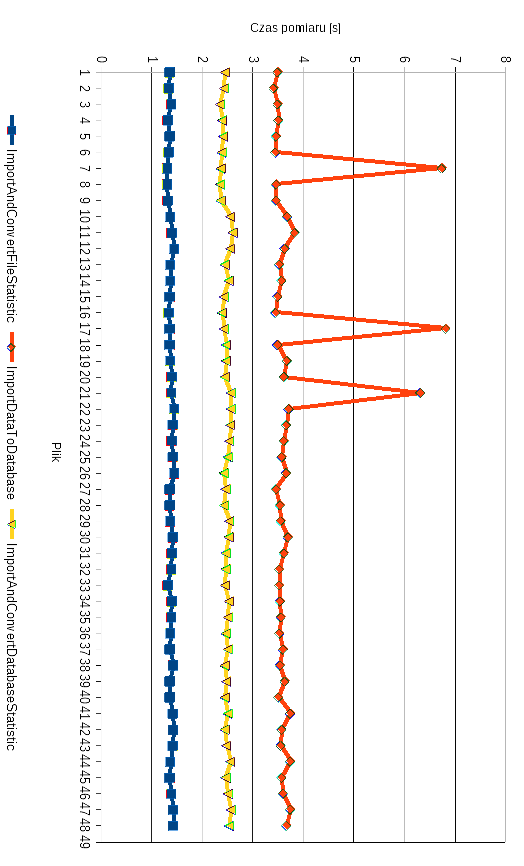
\includegraphics[width=\linewidth]{resources/statystyka_pomiaru.png}
    \caption{Przedstawienie wyników pomiaru czasu importu danych do aplikacji}
    \label{fig:importdata}
\end{figure}
\subsection{Porównanie końcowe algorytmów}
\label{ssec:compalgorithms}
Obserwując wyniki algorytmów zaprezentowane w sekcji \ref{ssec:queryparameters} wyniki końcowe zależą dużo od wartości parametrów wejściowych algorytmów. Niepoprawna wartość prędkości granicznej dla algorytmu I-VT, czy też wartości dyspersji i rozmiaru czasowego okna dla algorytmu I-DT może powodować zbyt duże nagromadzenie, lub wręcz przeciwnie zbyt małą ilość danych. Dlatego niezbędne jest znalezienie w ciągu weryfikacji danych, jeżeli istenieje taka możliwość odpowiedniej wartości tych parametrów.\par
Jak już zostało napisane w sekcji \ref{sssec:ivtresults}, w trakcie testów odkryto, iż prawidłowy parametr prędkości mieści się w przedziale $v \in (0,0001;0,001)$. Jest to spowodowane dokładnością urządzenia pomiarowego i wykonanego nim pomiaru. Należy ten parametr dostosowywać w zależności od wykonanego pomiaru. Przykładowe wyniki tego algorytmu odpowiednio dla wartości parametru \emph{v} wynoszących \emph{0.00001, 0.0005} oraz \emph{0.005} i \emph{0.05} dla pliku \emph{1\_03\_1310301904.cal} zaprezentowano w odpowiedniej kolejności na rysunkach \ref{fig:ivt1}, \ref{fig:ivt2}, \ref{fig:ivt3}, \ref{fig:ivt4}. Można na nich zaobserwować potwierdzenie powyższego założenia. Patrząc na tabelę  wartości fiksacji wynoszą 11763, 2801, 35, 1. Zastanawiającym wynikiem analizy jest różnica w ilości punktów w linii do punktów $P_1 = (0.95,0.5)$ oraz $P_2 = (0.95, 0.025)$. Dla rysunku \ref{fig:ivt1} i \ref{fig:ivt2} możemy zaobserwować zmianę ilości punktów w linii, ale zwiększona jest ilość punktów w fiksacji dla punktów skupionych przy wartościach 'RR'. Być może dla tego pliku został w danych wyraźnie zaznaczony ruch oka.\par
Nie jest zaskakującym wynikiem czas trwania algorytmu, wraz z wykorzystaniem pamięciowym, gdyż jedno porównanie do następnego elementu w tablicy, w wypadku poprawnie skonstruowanego kodu nie powinno stanowić dużej złożoności czasowej oraz pamięciowej.
\begin{figure}[H]
    \centering
    \captionsetup{justification=centering,margin=2cm}
    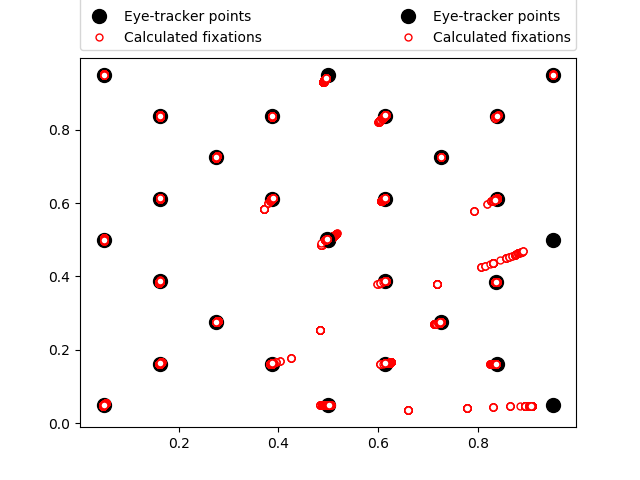
\includegraphics[width=0.8\linewidth]{resources/ivtresults/file1.png}
    \caption{Wynik algorytmu I-VT dla v = 0.00001}
    \label{fig:ivt1}
\end{figure}
\begin{figure}[H]
    \centering
    \captionsetup{justification=centering,margin=2cm}
    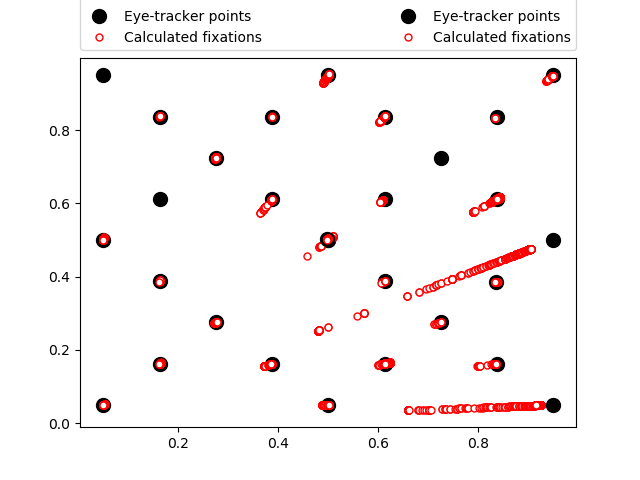
\includegraphics[width=0.8\linewidth]{resources/ivtresults/file2.png}
    \caption{Wynik algorytmu I-VT dla v = 0.0005}
    \label{fig:ivt2}
\end{figure}
\begin{figure}[H]
    \centering
    \captionsetup{justification=centering,margin=2cm}
    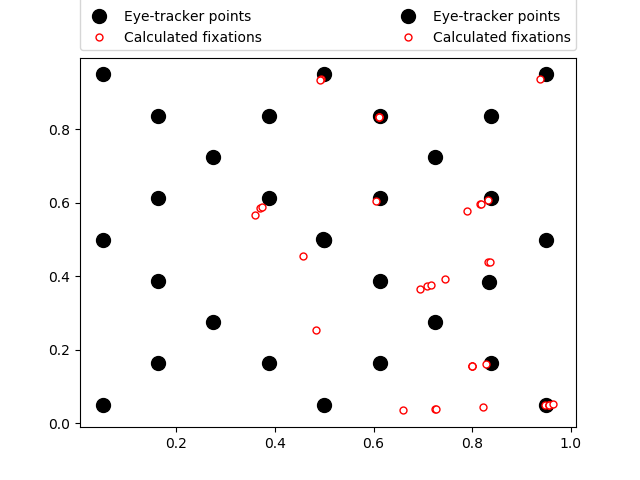
\includegraphics[width=0.8\linewidth]{resources/ivtresults/file3.png}
    \caption{Wynik algorytmu I-VT dla v = 0.005}
    \label{fig:ivt3}
\end{figure}
\begin{figure}[H]
    \centering
    \captionsetup{justification=centering,margin=2cm}
    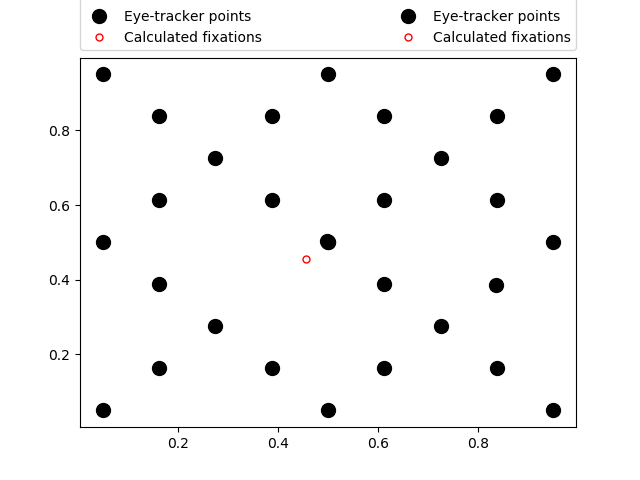
\includegraphics[width=0.8\linewidth]{resources/ivtresults/file4.png}
    \caption{Wynik algorytmu I-VT dla v = 0.05}
    \label{fig:ivt4}
\end{figure}
Pierwszym wnioskiem z analizy pracy algorytmu I-DT jest to, iż jest on najdłużej działającym algorytmem.\par
Dla algorytmu uczenia maszynowego zaskakującą informacją jest to, że zauważono brak znaczącego wpływu na wyniki końcowe przez to ile procent danych przeznaczono na testy a ile na trening modelu. Również nietypowym zjawiskiej jest odwrotność ilości wykrywanych fiksacji względem algorytmu I-VT, który posłużył za przygotowanie liczby wynikowej. Celem dokładniejszej analizy tych algorytmów należałoby posiadać dane, które posiadałyby już określoną wartość klasy przynależności do grupy, gdyż błędny parametr zgodnie z pierwszym paragrafem może powodować niedokładne wyniki. Być może też posiadanie takich danych pozwoliłoby na wyeliminowanie problemu pustych wyników w tabelach znajdujących się w paragrafie \ref{sssec:mldivide} i \ref{sssec:mlivt}.